\section{Einleitung}
Der bipedale Gang des Menschen ist ein Erkennungsmerkmal unserer Fortbewegung und weist ein Alleinstellungsmerkmal gegenüber anderer bipedalen Bewegungsstilen auf: die fast vollständige Streckung der Beine (ALEXANDER 1992). Die Erforschung der menschlichen Fortbewegung erstreckt sich dabei von der Ganganalyse (alexander und wer noch so alles) über klinische Forschung (WREN ET AL 2011) bis hin zur Untersuchung von Laufmustern für Roboter (TLOK-XXX und ...noch eins..).
Um den Gang genauer zu untersuchen wird der Gangzyklus grundlegend unterteilt in Standphase und Schwungphase sowie weitere Sub-Phasen, die in Abbildung \ref{fig:Skizze_Phasen} dargestellt sind (Perry XXX).\\
Der Menschliche Gang lässt sich dabei sehr gut mit dem Modell eines inversen Pendels abstrahieren. Durch das fast vollständig gestreckte Standbein rotiert die Hüfte um den Kontaktpunkt mit dem Boden. Das Schwungbein verhält sich dagegen wie ein normales Pendel und schwingt um die Hüfte. Mit der Distanz des Beinschwerpunktes bis zur Hüfte lässt sich das Bein als mathematisches Pendel abstrahieren und so die Eigenfrequenz des Beines bestimmen. Bewegt man sich mit der Geschwindigkeit fort, bei der das jeweilige Schwungbein mit dieser Periodendauer schwingt, ist für die Beinbewegung keinerlei Energie notwendig (KUO 2007, HIER VLLT ANDERE QUELLE?!?!).\\
%Betrachtet man Standbein und Schwungbein zusammen, dürfte die Fortbewegung keine Energie benötigen. Dieses Paradoxon wird durch Abweichungen von einem ideal gestreckten Bein sowie einer Bremskraft beim initialen Bodenkontakt erklärt (KUO 2007). (DEN ABSATZ WAHRSCHEINLICH LÖCSHEN!)\\
Das Modell des inversen Pendels kann durch den subjektiven Energieaufwand beim Gehen überprüft werden. Bewegt man sich mit genau der richtigen Geschwindigkeit fort, sollte das Laufen als sehr angenehm empfunden werden und ohne großen Kraftaufwand möglich sein.
\begin{wrapfigure}{r}{6cm}
	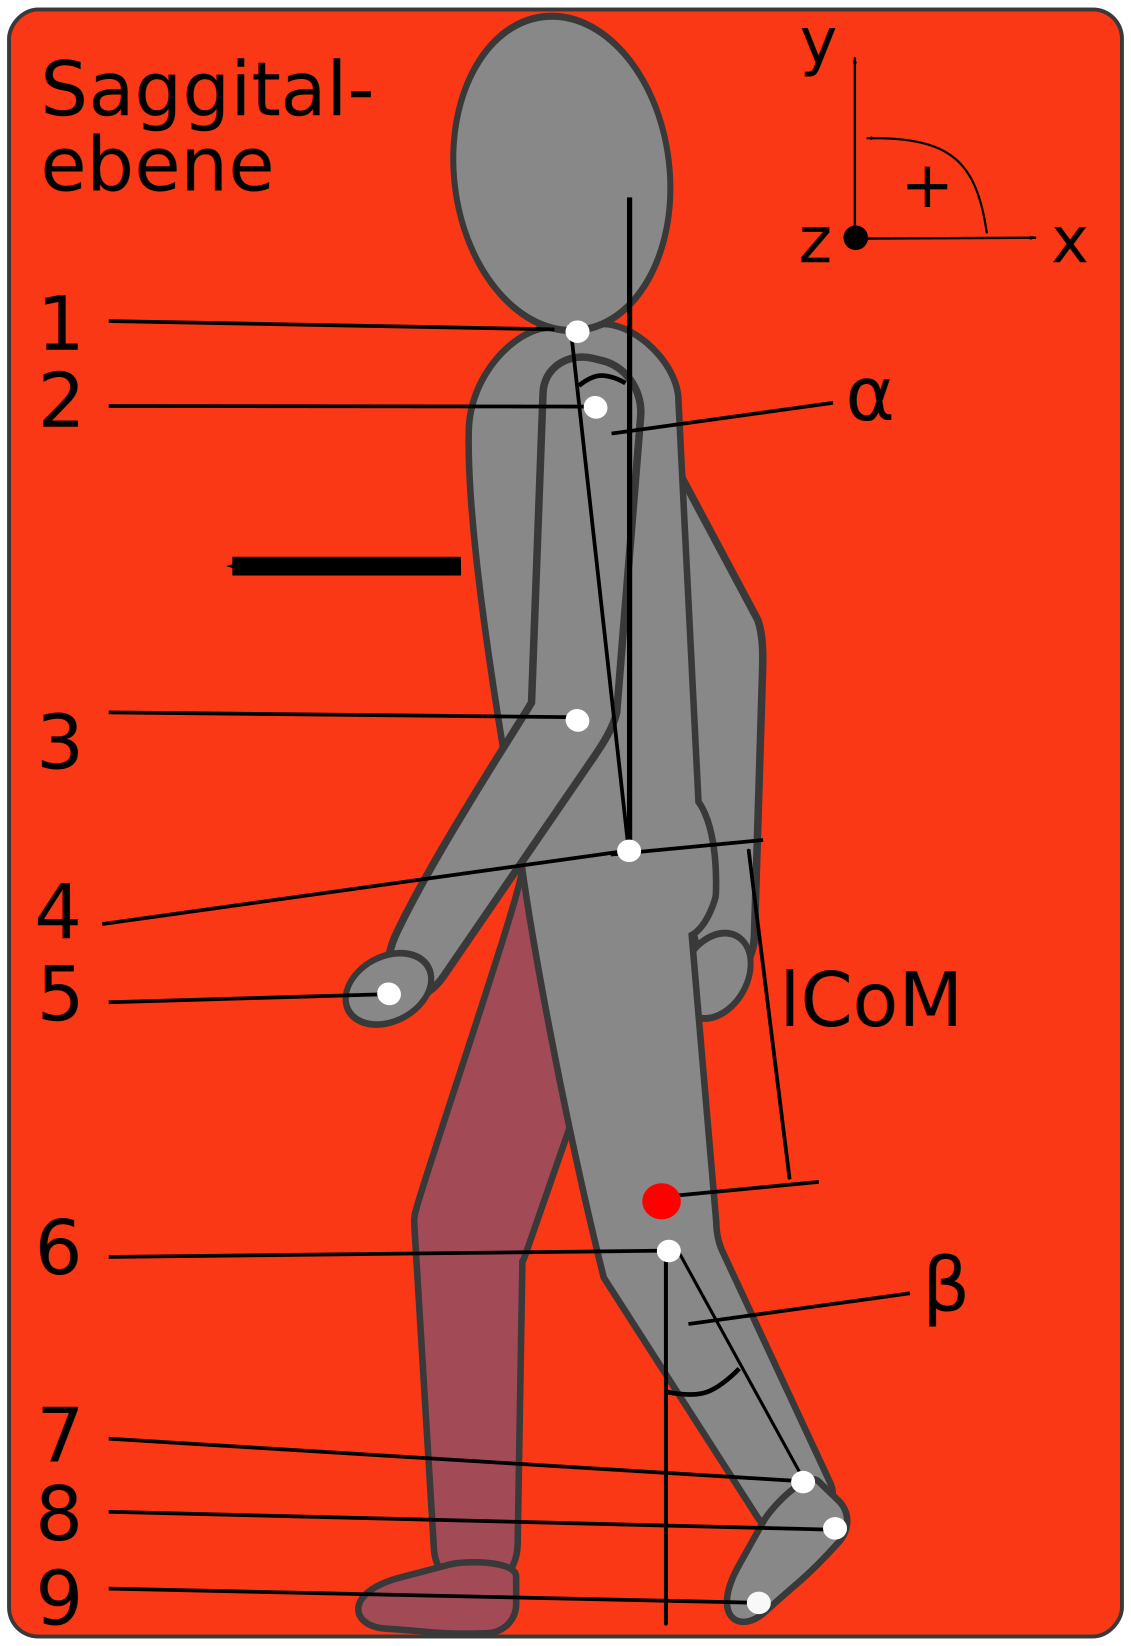
\includegraphics[width=\linewidth]{bilder/Einleitung/Proband_Pendel}
	\caption[Inverses Pendel und untersuchte Gelenke]{Untersuchungsebene, wichtige Gelenke (weiße Kreise), Länge des virtuellen Pendels ($l_{CoM}$) von Hüfte bis zum Massenschwerpunkt des Beines (roter Kreis) sowie Neigungswinkel des Oberkörpers zur Senkrechten ($\alpha$)}
	\label{fig:Proband_Pendel}
\end{wrapfigure}
Weitere Aussagen über den Gang lassen sich durch das Messen der Bodenreaktionskräfte (BRK) treffen. Verbindet man diese mit der kinematischen Analyse können Momente wie Lastaufnahme in Y-Richtung sowie ein Abbremsen und Abstoßen in X-Richtung beobachtet werden. Die Kräfte in Z-Richtung erlauben Aussagen über die Balance beim Gehen, welche besonders interessant sind für die monopedalen Stützphasen (ehhh, QUELLE?).
Ziel dieser Arbeit ist die exemplarische Datenerhebung mittels kinematischer und kinetischer Verfahren für einen Probanden. Das Gehen wird bei verschiedenen Geschwindigkeiten untersucht und eine allgemeine Auswertung von Periodendauer durchgeführt, um die Theorie des inversen Pendels zu testen. Die Versuche auf dem Laufband und der Laufstrecke werden auf Unterschiede in der Körperneigung und der Handtrajektorie verglichen. Unterschiede zwischen den beiden Experimenten könnten auf eine Anpassung des Gehens an die tatsächliche Ortsänderung auf der Laufstrecke sein. Zusammen mit den Kraftmessungen werden mittels inverser Kinematik auf der Laufstrecke die auftretenden Kräfte und Momente in Knöchel, Knie und Hüfte untersucht und hier Aussagen zu ( JA ZU WAS DENN?? LAUFROBOTER??, BESSERE SCHUHE??) abgeleitet. Alle ermittelten Daten werden mit der Literatur verglichen und die Experimente auf ihre Belastbarkeit geprüft, da auf eine statistische Belastabrkeit der Messdaten verzichtet wurde, um den Umfang der Untersuchungen zu erhöhen.\\
HIER NOCH ABBILDUNG DES PROBANDEN MIT PENDEL ETC EINBINDEN!!

\begin{figure}
	\centering
	\includegraphics[width=\linewidth]{bilder/Einleitung/Skizze_Gangphasen_small}
	\caption[Gangphasen]{blabla blabla}
	\label{fig:Skizze_Phasen}
\end{figure}





\begin{figure}
	\centering
	\includegraphics[width=0.7\linewidth]{bilder/Einleitung/gangphasen}
	\caption[Gangphasen]{blabla blabla}
	\label{fig:gangphasen}
\end{figure}